\documentclass[11pt,a4paper, uplatex]{jsarticle}
%
\usepackage{amsmath,amssymb}
\usepackage{bm}
\usepackage[dvipdfmx]{graphicx}
\usepackage{ascmac}
\usepackage{listings,jlisting}
\usepackage{underscore}
\usepackage{subfig}
\lstset{
    frame=single,
    numbers=left,
    tabsize=2
}
%
\setlength{\textwidth}{\fullwidth}
\setlength{\textheight}{40\baselineskip}
\addtolength{\textheight}{\topskip}
\setlength{\voffset}{-0.2in}
\setlength{\topmargin}{0pt}
\setlength{\headheight}{0pt}
\setlength{\headsep}{0pt}
%
\newcommand{\divergence}{\mathrm{div}\,}  %ダイバージェンス
\newcommand{\grad}{\mathrm{grad}\,}  %グラディエント
\newcommand{\rot}{\mathrm{rot}\,}  %ローテーション
%
\title{メディア情報学実験・音声認識 第三週課題レポート}
\author{1510151  栁 裕太}
\date{\today}
\begin{document}

\maketitle
\section{認識対象の単語}
\begin{table}[htbp]
  \begin{center}
    \caption{実験で使用した数字単語}
    \label{tb:numbers}
    \begin{tabular}{c|c|c|c}
      \hline
      単語表記 & 単語名 & 発音 & 音素数 \\ \hline \hline
      3 & saN & /saN/ & 3 \\
      4 & yoN & /yoN/ & 3 \\
      5 & go & /go/ & 2 \\
      7 & nana & /nana/ & 4 \\
      \hline
    \end{tabular}
  \end{center}
\end{table}

\section{HMMの学習曲線}

\begin{figure}[h]
  \begin{center}
    \includegraphics[width=13.0cm]{learningCurve.ps}
    \caption{実行結果グラフ(go)}
    \label{fig:ps}
  \end{center}
\end{figure}

\section{単語認識性能評価}
\subsection{自分の声}
\subsection{他人の声}

\section{オンライン単語認識}
\subsection{自分の声}
\subsection{他人の声}


\section{実験のポイント}


\section{よくわかったこと}


\section{よくわからなかったこと}


\section{要望}

\section{感想・その他}

\end{document}
